\section{Register description}
\regover{
{\hyperref[pds-PDS-CTL]{PDS\_CTL}}&
\\
\hline
}

\subsection{PDS\_CTL}
\label{pds-PDS-CTL}
Address:0x2000e000
 \begin{figure}[H]
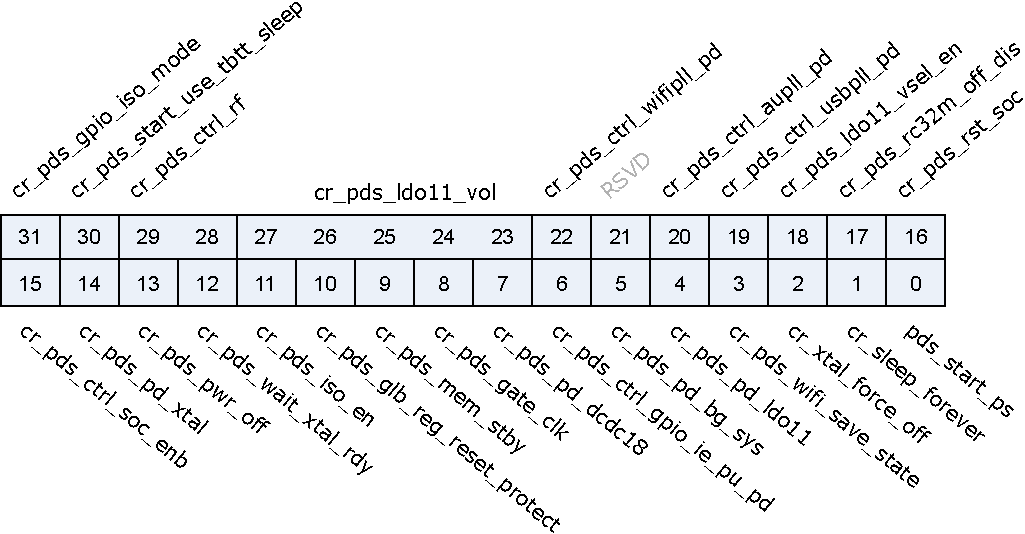
\includegraphics{pds_PDS_CTL.pdf}
\end{figure}

\regdes{31:1&RSVD& & & \\\hline
0&pds\_start\_ps&w1p&0&Enter PDS\\\hline
-1:22&RSVD& & & \\\hline
21:16&cr\_pds\_ram\_clk2\_cnt&r/w&6'd24&HW Option : Assert Extra Clock Counter in MEM\_IDLE\\\hline
15:19&RSVD& & & \\\hline
18:16&cr\_pds\_gpio\_keep\_en&r/w&3'b111&if cr\_pds\_gpio\_iso\_mode=1, can use bit to enable or disable keep function \par [0] : LEFT Side PAD (GPIO0~8, GPIO44,GPIO45) \par [1] : Right side PAD (GPIO16~23, GPIO42, GPIO43) \par [2] : TOP Side PAD (GPIO24~39)
\\\hline
15:10&RSVD& & & \\\hline
9&cr\_pds\_pd\_ldo18io&r/w&0&0 : don’t\_touch ldo18io during PDS \par 1 : power down ldo18io during PDS
\\\hline
8&cr\_pds\_ctrl\_usb33&r/w&0&Set this bit to enable HW control turn on/off USB 3.3V @USB1.1V Power On/OFF \par (Replace the function of reg\_pu\_usb20\_psw)
\\\hline
7:0&RSVD& & & \\\hline

}
